\chapter{The Easy Service Creation Perspective}
\label{sec:user_perspective}

This section will briefly introduce those parts of the Eclipse GUI that are relevant for the work with the Visual Service Design Tool.  These views are aggregated in the Easy Service Creation perspective, which an be selected via the Menu \emph{Window $\rightarrow$ Perspective}.  Figure~\ref{fig:screen} (page~\pageref{fig:screen}) is showing a screenshot of the Visual Service Design Tool featuring most of the relevant views.  In the following each of the views will be introduced briefly.


\section{VSDT Editor Views}
\label{sec:user_perspective_editor}

The editor window is shown automatically when opening a file in the Navigator view. Depending on the PlugIns currently installed this can be a plain text editor, a browser, an elaborate code editor or some sort of graphical editor. For the Visual Service Design Tool there are two editors available: A visual editor showing the BPMN graph and a tree editor reflecting the internal structure.  

\paragraph*{The Graphical Editors}
These are the primary editors when working with the VSDT (see Figure~\ref{fig:screen_meta}):

\begin{figure}
	\centering
	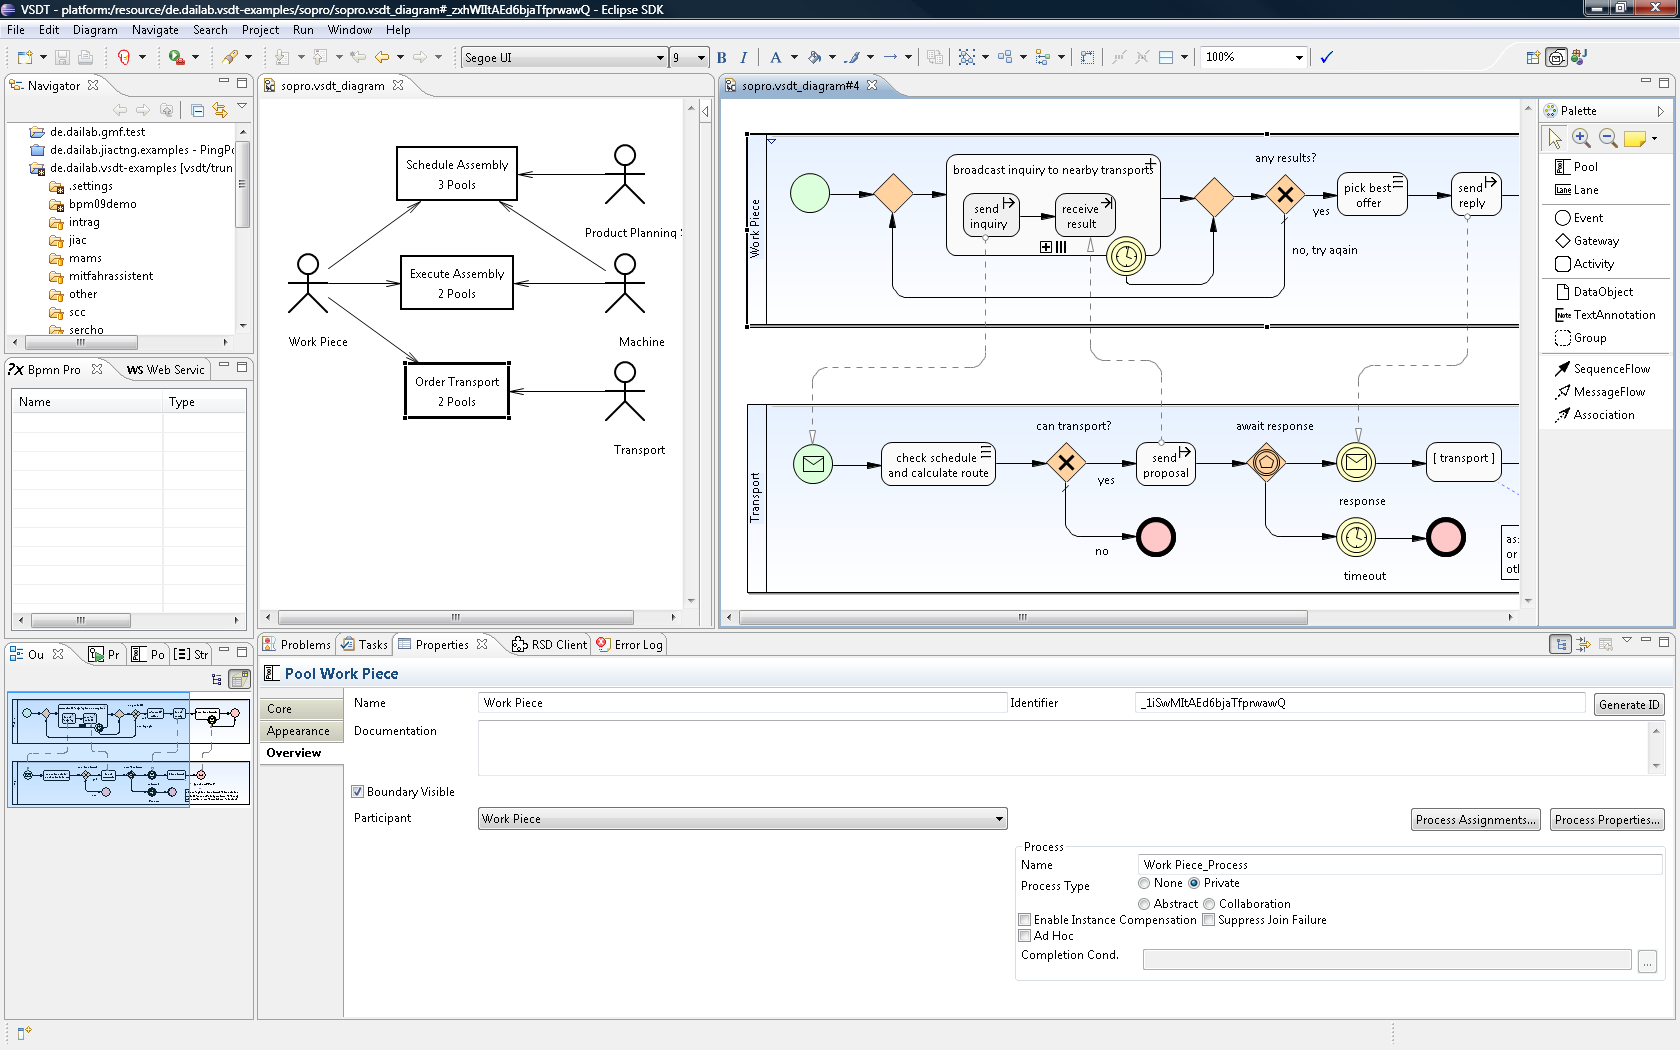
\includegraphics[height=.4\textheight]{figures/vsdt_1-2-0.png}
	\caption{Business Process System and BPMN editor shown side-by-side.}
	\label{fig:screen_meta}
\end{figure}

\begin{itemize}
	\item The \emph{Business Process System} editor is opened when the diagram file is clicked.  It is used for organizing the several interdependent Business Processes which make up the system as a whole, as well as the Participants involved in these Processes.
	\item The \emph{Business Process Diagram} editor is opened when double-clicking one of the Business Process Diagram nodes in the Business Process System editor.  This editor is the actual BPMN editor used for modelling the individual Business Processes.
\end{itemize}

Both editors feature a palette with the nodes and connections. For placing a node on the canvas or inside a compartment of another node (e.g. a Pool or a Sub Process) click the icon in the palette and then click again on the canvas.  For drawing connections, click on the first node, draw the connection to the second node and release the mouse button. Note that nodes and connections can not be drawn arbitrarily, but have to follow the BPMN syntax, e.g. a Task can only be drawn inside a Pool and a Sequence Flow can only connect Flow Object within the same Pool.

\paragraph*{The Tree Editor}
The tree editor can be useful for managing and editing those parts of the Business Process Diagram that do not have a graphical representation.\footnote{Although in general it is not necessary to use the tree editor, as the graphical editor provides means for editing non-graphical elements, too.}  Note that the tree editor is more powerful than the graphical editor, and the diagram might be invalidated when doing certain operations in the tree editor.  Especially, the tree editor should \emph{not} be used for creating any elements that \emph{do} have a graphical representation in the diagram, as this representation will not be created along with the element.  In case the diagram file is broken, it can be recreated from the model file by right-clicking it and selecting the respective menu item.

\paragraph*{The Text Editor}
Both the diagram and the model file can be opened with any text editor and edited as XML.  While this can be helpful for adapting existing models to changes in the metamodel of a newer version of the VSDT, you should in general avoid editing the files XML sources, as this can render them unreadable for the other editors.



\section{General-purpose Eclipse Views}
\label{sec:user_perspective_general}

In the following those standard views of the Eclipse IDE will be introduced, that are relevant for the work with the VSDT.

\paragraph*{The Navigator}
Here the user can manage his projects and create and delete files.  Note that Eclipse provides different similar views for managing files, e.g. the Navigator, Project Explorer or the Package Explorer, each providing slightly different features.

\paragraph*{The Properties View}
Although some attributes, like an element's name, can be edited in the graphical editor view as well, for most other attributes the properties view will be needed, where all the attributes relevant to the user can be inspected and edited. Of course, each change done in the properties view can be undone and redone and the editor will be immediately updated. There are two tabs available in the properties view: The \emph{Core} tab provides a table showing the attributes in categories and in alphabetic order. The \emph{Overview} tab provides a clearer look, grouping the attributes and arranging them by relevance in two columns. Additionally, the Outline tab features a number of buttons, providing access to additional dialogs for managing e.g.\ an Activity's Properties and Assignments.

\paragraph*{The Outline}
This view provides a short outline of the current editor's content. In case of a graphical editor, like the VSDT, this can be a miniature view of the entire diagram, and in case of a tree editor an additional tree view for easier navigation. 

\paragraph*{The Problem View}
This view lists all the problems that have been found in the model, subdivided in errors and warnings. By double-clicking one of the items the editor will focus on the element the problem occurred on (for refreshing the errors shown in the Problem View, select \emph{Diagram | Validate} from the menu).

\paragraph*{The Error Log}
Other than the Problem View, the Error Log will log problems with the editor itself. So if you encounter strange behaviour or in case the editor should crash you can check here for the reason and send in an error report.



\section{Additional Views for the VSDT}
\label{sec:user_perspective_custom}

The following are views that have been crafted especially for the VSDT.


\paragraph*{The BPMN-Properties View}
\label{sec:user_perspective_propView}

The BPMN-Properties View (see Figure~\ref{fig:customViews}, to the left) provides an easy way to inspect the Properties in the scope of the currently selected element in the active editor, i.e. the Properties that can be used in an Assignment owned by that element. The property scope of a BPMN element comprises the Properties of (a) that element itself, e.g. an Activity, (b) Messages going in and out of that element, e.g. the in- and output parameters of a Web service call, and (c) the (transitive) parents of that element, e.g. (Sub-) Processes.

\begin{figure}[t]
	\centering
	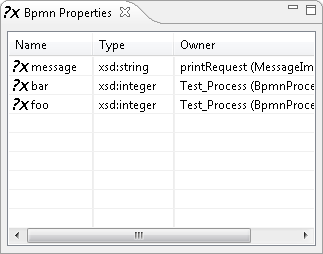
\includegraphics[width=.3\textwidth]{figures/features/propView.png}
	\hspace{.5cm}
	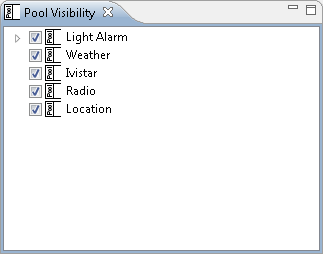
\includegraphics[width=.3\textwidth]{figures/features/poolView.png}
	\hspace{.5cm}
	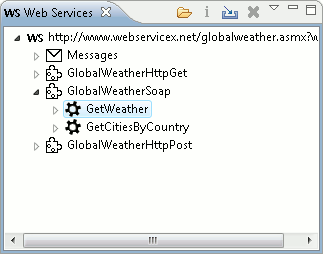
\includegraphics[width=.3\textwidth]{figures/features/wsView.png}
	\caption{The BPMN Properties View, Pool Visibility View, and Web Service View.}
	\label{fig:customViews}
\end{figure}

The Properties are displayed in three columns, showing the name and the type of the Property and the name and the element type of the Property's parent element. The properties an be sorted by clicking on the column heads.  By double-clicking on a Property, an Organize Properties Dialog will be opened for the Property's parent element.


\paragraph*{The Pool Visibility View}

In the Pool Visibility View, which is seen in the centre of Figure~\ref{fig:customViews}, all the Pools in the diagram are displayed.  If the check box in front of an entry is unchecked, the corresponding Pool and all incoming and outgoing connections, e.g.\ Message Flows, will be hidden.  This feature can be of some use in diagrams holding many Pools:  When modelling three or more interconnected Pools, Message Flows going from the first to the third Pool might cross the second Pool, which can be confusing when editing that Pool.  In this case, the first or the third Pool may be hidden, so the Message Flows (which are then hidden, too) do not longer obstruct the view on the second Pool.  In the same way the Pools and Message Flows can be shown again by checking the corresponding check box.  Note that these settings are not persisted, so when closing and re-opening a diagram all Pools will be visible again.  %Further, the Pool entries can be expanded, showing an outline of the elements within. However, this feature, which might some day supplement the Outline View, is still at an early stage.


%\paragraph*{The RSD View}
%The RSD view can be used to inspect and import Web services into the process diagram.  Using the RSD View not a single Web service is inspected, but the content of a \emph{Rich Service Directory}, a special kind of Web service repository also capable of advertising services and operations from other sources, e.g. UPnP devices or JIAC TNG actions.  The several operations of each Web service registered at the Rich Service Directory are displayed in a list from which they can be selected, inspected, and imported into the diagram. When importing Web services, the corresponding Web service descriptions and input and output messages will be created automatically.  However, the RSD implementation is still at an early stage, and thus by now the use of the RSD View is limited.


\paragraph*{The Web Service View}
%Similar to the RSD View, this view can be used to inspect and import Web service descriptions into the active BPMN diagram. However, other than using the RSD view, the Web Service view does not need the RSD but will directly connect to a given Web service URL.
The Web Service View (see Figure~\ref{fig:customViews}, to the right) provides access to Web Services, which can be inspected and imported into the currently opened diagram.  Web Services can be added to the list by clicking the Open button and entering the exact URL of the WSDL definitions file.  The Web Service is displayed as a tree, including the various Messages and their types, nad the Port Types, their Operations, and their In- and Output Messages.  By clicking the Info button, the complete WSDL definition is shown in plain XML. Most importantly, Messages and Operations can be imported from the Web service description into the Business Process Diagrams, so they can be reused in a Web service invocation.


\paragraph*{The Interpreter View}
\label{sec:user_perspective_simView}
BPMN diagrams created with the VSDT can be simulated and interpreted using the built-in process interpreter (see Figure~\ref{fig:customViews2} and Section~\ref{sec:user_features_sim}).  For starting a simulation, first switch to the BPMN diagram you want to simulate. Open the Process Interpreter View and click the \emph{Start} button.  For each Pool in the diagram, the view will show those Activities that are currently \textsc{active} or \textsc{ready}.  For advancing a step in the simulation, expand a Pool and double-click one of the listed elements, that is the Flow Objects currently being ready, e.g.\ Start Events.  For more control, you can also select one of \emph{Step Over}, \emph{Step Into} or \emph{Step Out}.  Hit the Stop button for ending the simulation and removing the markers from the diagram editor view.

\paragraph*{The Structure View}
\label{sec:user_perspective_strucView}
This view allows to apply the Structure Mapping (see~\ref{sec:user_trafo_intro}) at modelling time, displaying the results in a tree.  By clicking on an element, the corresponding node in the diagram is highlighted.  Further, the user is notified if there seem to be structural conflicts in the process, which is determined from the number of left-over Sequence Flows.  This view should prove highly useful for validating the structure of processes prior to transformation to executable code (see Figure~\ref{fig:customViews2}).


\begin{figure}[t]
	\centering
	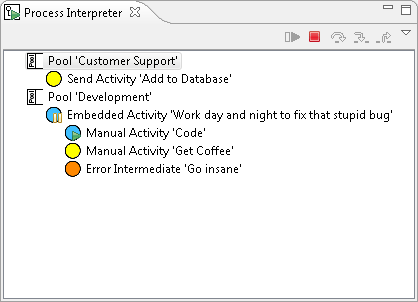
\includegraphics[width=.4\textwidth]{figures/features/interpreterView.png}
	\hspace{.5cm}
	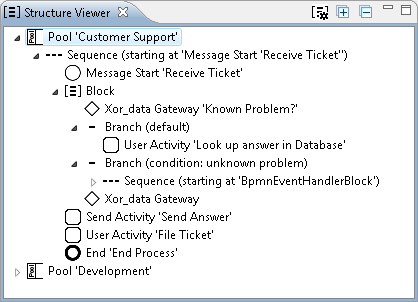
\includegraphics[width=.4\textwidth]{figures/features/structureView.png}
	\caption{The Interpreter View and Structure View.}
	\label{fig:customViews2}
\end{figure}
